\chapter{Appendix D}
\label{chap:appendix-d}
\section*{Installation Guide}
\label{sec:installation-guide}
This guide will outline the requirements and installation procedure to get the automation platform up and running. The guide will assume that the user has a basic understanding of Linux and the command line as well as Cisco ACI and VMware vCenter.

This solution is designed to allow a testing environment to provide OOB connectivity to a variety of projects within a testing environment through the use of a web UI. It achieves this through the use of Cisco ACI and VMware vCenter. Each rack within the lab space must have its own dedicated FEX or leaf switch as well as a terminal server, although a rack can exist without either. When racks are selected to be part of a project, the automation platform will deploy L2 connectivity to any FEX and leaf that belong to the selected racks, as well as including the terminal servers into this L2 domain. A virtual router will then be deployed on vCenter which will have the same aforementioned L2 connectivity to the selected FEXs and leafs, as well as connectivity to the desired WAN uplink. 

\section*{Requirements}
\begin{itemize}
    \item Cisco ACI v5.2(4d)
    \item VMware vCenter 7.0.3
    \item ESXi 7.0.3 Host (at least one)
    \item CSR1000v 17.03.05
    \item Terminal Servers (Must be IOS-XE 17.06.03a)
\end{itemize}

The solution will require some existing ACI configuration to be in place. The following will be required:

\begin{itemize}
    \item VMM integration between ACI and vCenter
    \item EPGs for terminal servers, internet connectivity, virtual routers and management VMs.
          \begin{itemize}
              \item The virtual router EPG must have a DHCP server to automatically assign IP addresses to the virtual routers.
          \end{itemize}
    \item An EPG that has access to the virtual router and terminal server EPGs, access to ACI and vCenter APIs can either be in-band or out-of-band.
    \item A static VLAN pool to be used by the automation platform, this should have a unique set of VLANs from any other VLAN pool to prevent issues from arising.
\end{itemize}

An example design of both the physical deployment and the ACI configuration can be seen in Figure \ref{fig:example-deployment} and Figure \ref{fig:example-aci} respectively.

\begin{figure}[H]
    \centering
    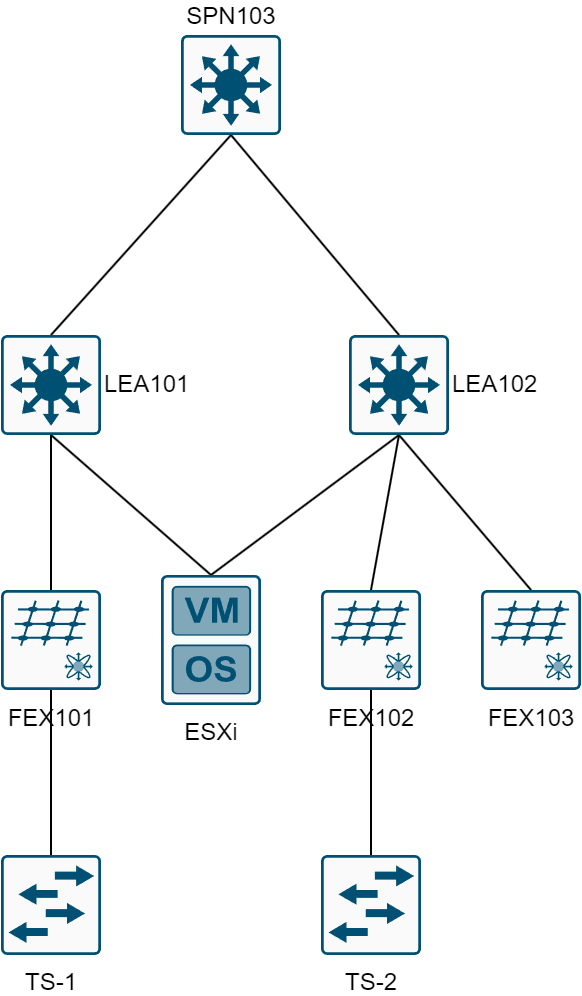
\includegraphics[width=0.5\linewidth]{images/aci-topology.png}
    \caption{Example physical deployment}
    \label{fig:example-deployment}
\end{figure}

\begin{figure}[H]
    \centering
    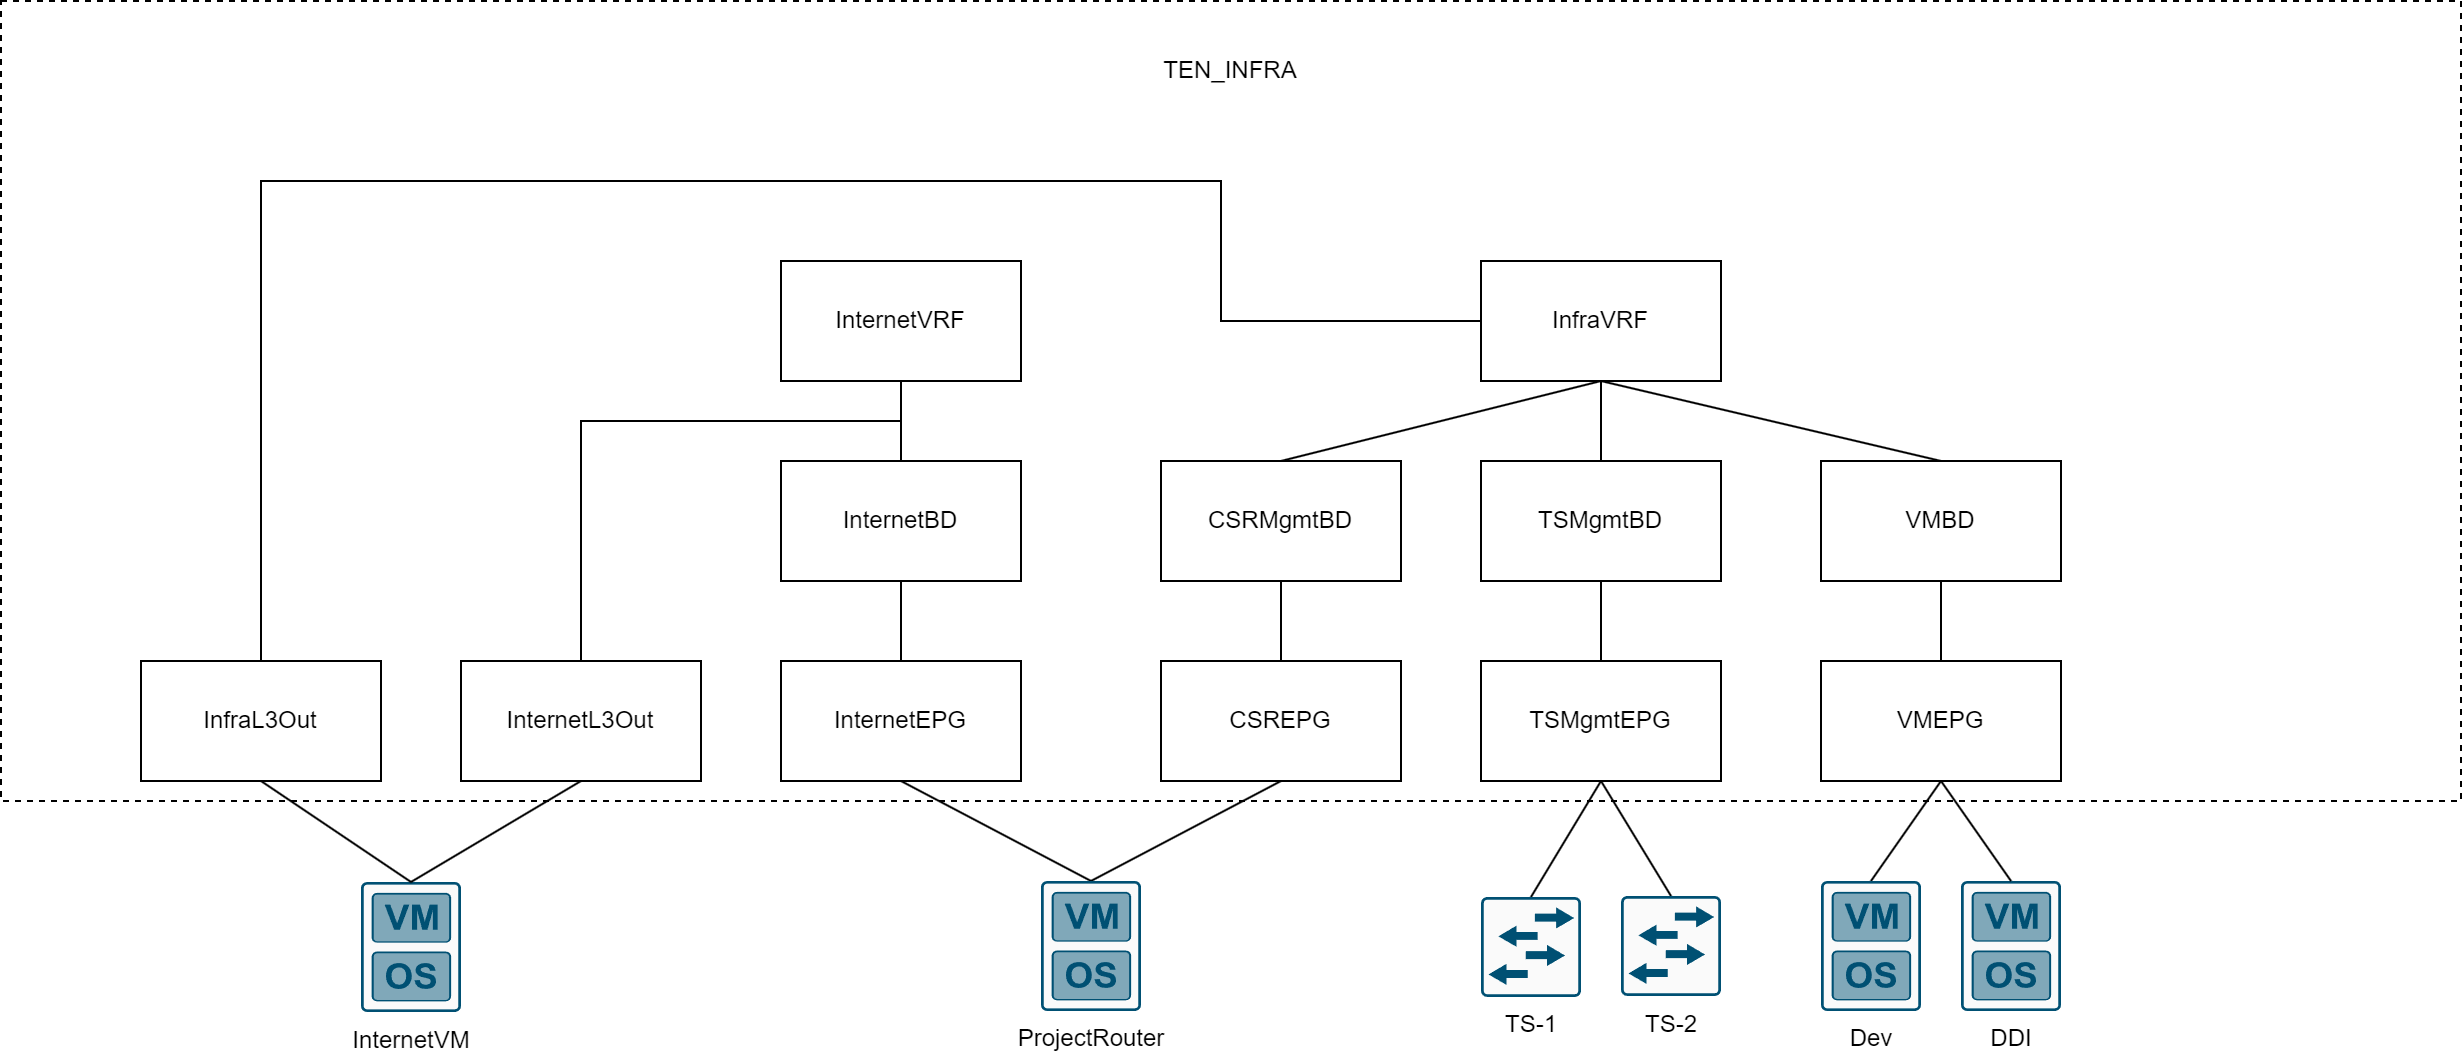
\includegraphics[width=1\linewidth]{images/epg-topology.png}
    \caption{Example ACI configuration}
    \label{fig:example-aci}
\end{figure}

\section*{ENV File Configuration}
For the automation platform to operate correctly, the .env file must be configured with the required information so that various services such as ACI and vCenter can be accessed correctly. A breakdown of the required .env file variables is provided below:
\begin{table}[H]
    \centering
    \begin{tabular}{l l p{0.4\linewidth}}
        \textbf{Variable}   & \textbf{Example} & \textbf{Description}                                                                                                \\
        \hline
        APIC\_IPADDR        & 192.168.0.125    & IP address of the APIC controller                                                                                   \\             \hline
        APIC\_USERNAME      & admin            & Username for the APIC controller                                                                                    \\            \hline
        
        APIC\_PASSWORD      & password         & Password for the APIC controller                                                                                    \\            \hline
        
        ACI\_POD            & 1                & The pod number of the ACI fabric that the automation platform will automate                                         \\            \hline
        
        ACI\_VMWARE\_DOMAIN & ACI-DVS          & The name of the VMM integration domain                                                                              \\            \hline
        
        ACI\_INFRA\_DOMAIN  & InfraPhys        & The name of the physical domain used to connect terminal servers to the ACI fabric                                  \\            \hline
        
        ENHANCED\_LACP      & LACP             & Name of the enhanced LACP policy used to connect ESXi nodes, leave this null if Enhanced LACP is not being utilised \\            \hline
        
        
        VSPHERE\_IPADDR     & 192.168.0.128    & IP address of the vCenter server                                                                                    \\            \hline
        
        VSPHERE\_USERNAME   & admin            & Username for the vCenter server                                                                                     \\            \hline
        
        VSPHERE\_PASSWORD   & password         & Password for the vCenter server                                                                                     \\            \hline
        
        PROJECT\_ROUTER     & ProjectRouter    & Name of the virtual router VM template                                                                              \\        
    \end{tabular}
\end{table}
